\chapter{Realisierung}

Im folgenden Abschnitt soll auf die Implementierung des \textit{Smart Warehouse} Szenarios eingegangen werden. Insbesondere werden Probleme während der Umsetzung der beiden Objektdetektoren \textit{SSD} und \textit{YOLO} betrachtet, Herausforderungen im Rahmen der Drohnen Anbindung besprochen und letztendlich die Realisierung der Dashboard-Webapplikation und des Zählalgorithmus zur Durchführung der Inventur aufgezeigt. 

\section{Umsetzung der Objektdetektoren}

\subsection*{SSD}

Für den \textit{SSD} wurde wie bereits erläutert nicht die ursprüngliche Referenzimplementierung im \textit{Caffe} Framework verwendet, sondern eine Custom-Implementierung in \textit{PyTorch}. Neben kleineren Änderungen in der Codebasis zur Erreichung von Kompatibilität mit aktuellen Bibliotheksversionen und weiteren Anpassungen zur Integration eines eigenen Datenbestandes, wurden vor allem zwei größere Erweiterungen durchgeführt. Da der erstellte Datenbestand nur 1078 gelabelte Daten enthält, wurde zusätzlich zur Custom-Implementierung ein fünffaches Kreuzvalidierungsverfahren realisiert. Es dient dazu ein höheres Abstraktionsvermögen des Modells auf dem geringen Datenbestand zu erreichen. Auch unterstützte die Referenzimplementierung keine Validierung durch zuvor ungesehene Daten. Die Modellklassen des Datenbestandes wurden dahingehend angepasst.

Um ein lokales Training auf der \textit{NVIDIA GTX 1080} GPU zu ermöglichen, wurde zudem \textit{CUDA} Version 10.1 verwendet. Trainiert wurde mit folgenden Hyperparametern:
\begin{itemize}
	\item Batch Größe: 16
	\item Lernrate: $1.0\cdot e^{-3}$
	\item Momentum: 0.9
	\item Epochen: 500
	\item Gradientenverfahren: Stochastic Gradient Descent
	\item Kostenfunktion: Smooth L1
\end{itemize}

Das Basisnetzwerk des \textit{SSDs} besteht aus einem auf \textit{ImageNet} vortrainierten \textit{VGG16}. Die restlichen \textit{Convolutional Layer} sind \textit{Xavier} initialisiert. 

Die Hyperparameter sind nahezu gleich zu denen in der ursprünglichen wissenschaftlichen Veröffentlichung. Wesentlich die Batch Größe wurde für größere Stabilität von 32 auf 16 heruntergesetzt. Auch in der Evaluierung wurde die Batch Größe von 64 auf 48 herunter gesetzt, da die Eingangsdaten eine weitaus höhere Auflösung als die ursprünglich im \textit{PascalVOC} verwendeten Daten haben. Andernfalls wird Gefahr gelaufen einen Speicherüberlauf zu erzielen. 

Ursprünglich wurden 500 Epochen für das Training vorgesehen für jeden der Kreuzvalidierungsschritte. Da allerdings beim Training schon nach knapp über hundert Epochen sich der Gradient der Kostenfunktion nur träge veränderte, wurde im Sinne des \textit{Early Stoppings} nach 108 Epochen das Training vorzeitig beendet, um \textit{Overfitting} zu vermeiden. Das niedrigste Ergebnis der Kostenfunktion betrug 1.726. Es ergab eine \textit{mAP} von 78.25\%, leicht über den Referenzergebnissen von \textit{SSD} zu \textit{PascalVOC} (siehe Abbildung \ref{result}). Die Ergebnisse zu den einzelnen Klassen sind in folgender Tabelle dargestellt:

\begin{center}
	\begin{tabular}[h]{l|c}
		Klasse & mAP \\
		\hline
		Saskia Wasser Groß & 77.62\% \\
		Saskia Wasser Klein & 75.96\% \\
		Pepsi Cola Groß & 25.715\% \\
		Pepsi Cola Klein & 50.00\% \\
		ISO & 100.00\% \\
		ACE & 100.00\% \\
		Stenger Johannisbeerschorle & 100.00\% \\
		Stenger Apfelsaftschorle & 100.00 \% \\
		Vitamalz Malzbier & 75.00\%
	\end{tabular}
	\captionof{table}{Validierungsergebnisse SSD}
	\label{table:ssdresults}
\end{center}

Wird nun das trainierte Modell auf echte Daten angewendet, so fällt auf, dass manche Objekte doppelt detektiert werden. Um dieses Problem zu lösen, gibt es zwei Möglichkeiten. 

Als erstes kann bei der Detektion der minimale \textit{confidence score} angegeben werden, ab wann eine Detektion offiziell als solche wahrgenommen wird. Hier liegt die Herausforderung darin, einen optimalen Wert zu finden, sodass verdeckte Objekte noch als solche erkannt werden, aber doppelt erkannte Objekte nicht mehr auftreten. Der \textit{confidence score} wurde nach mehrmaligem Iterieren auf 0.75 festgelegt.

Die zweite Möglichkeit besteht darin, die maximale Überlappung zweier Bounding Boxen festzulegen. Somit werden doppelte Bounding Boxen, die sich flächenmäßig über einem gewissen Grenzwert überlappen, auf eine Bounding Box reduziert. Er stellte ich sich Parameter von 0.5 als geeignet heraus.

Außerdem wurden Inkonsistenzen im Detektionsverhalten festgestellt:

\begin{figure}[ht]
	\centering
	\subfigure[verdeckt]{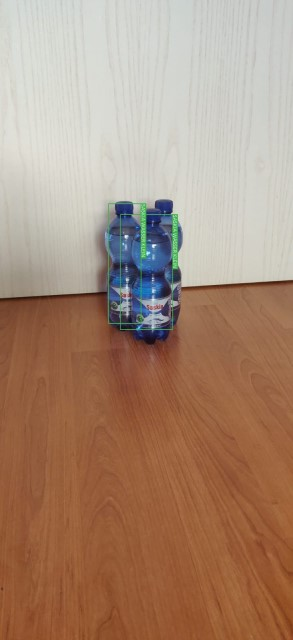
\includegraphics[width=0.30\textwidth]{Bilder/verdeckt.jpeg}}
	\hspace{2cm}
	\subfigure[winkel]{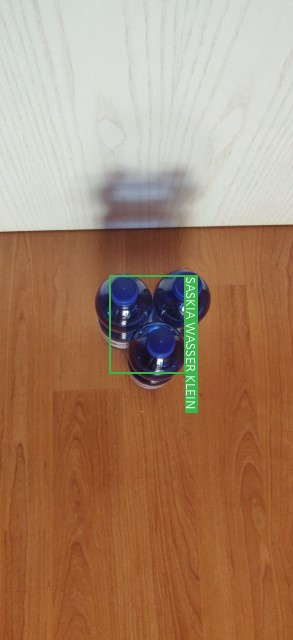
\includegraphics[width=0.30\textwidth]{Bilder/winkel.jpeg}}
	\caption{Detektionsverhalten bei extremen Blicklagen}
	\label{lagen}
\end{figure}

So sind von anderen Objekten verdeckte Objekte nur schwer zu erkennen, genauso wie Objekte aus extremen Blicklagen (siehe Abbildung \ref{lagen}). Diese Fälle wurden im Datensatz zwar zu 12.5\% abgedeckt, es lässt sich aber keine Aussage darüber treffen, ob eine Erweiterung des Datensatzes eine Abhilfe für dieses Problem hätte liefern können. 

\begin{figure}[ht]
	\subfigure[1 Meter]{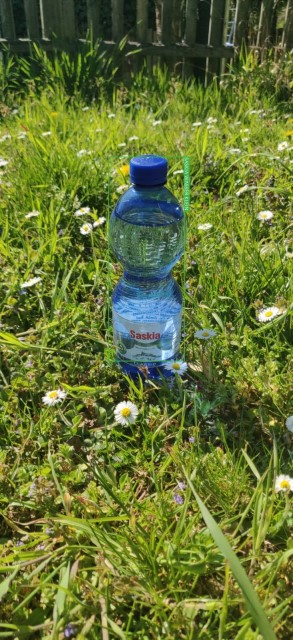
\includegraphics[width=0.30\textwidth]{Bilder/einmeter.jpeg}}\hfill
	\subfigure[2 Meter]{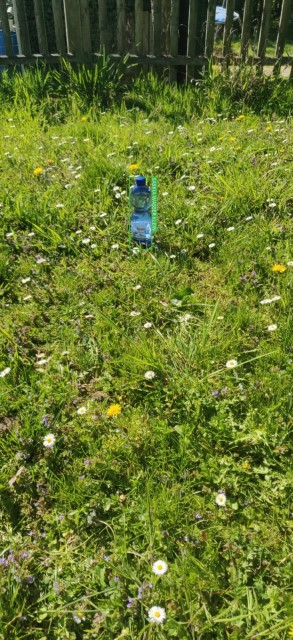
\includegraphics[width=0.30\textwidth]{Bilder/zweimeter.jpeg}}\hfill
	\subfigure[3 Meter]{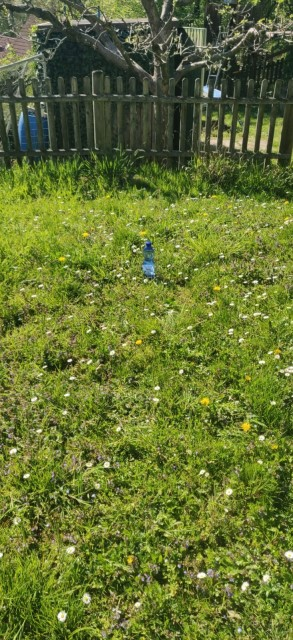
\includegraphics[width=0.30\textwidth]{Bilder/dreimeter.jpeg}}\hfill
	\caption{Detektionsverhalten bei unterschiedlichen Entfernungen}
	\label{entfernung}
\end{figure}

Auch die Entfernung zum zu detektierenden Objekt besitzt eine Auswirkung auf das Detektionsverhalten. In Abbildung \ref{entfernung} wird gezeigt, dass ab einer Entfernung von drei Metern keine Detektion mehr erfolgte. 

\begin{figure}[ht]
	\subfigure[überbeleuchtet]{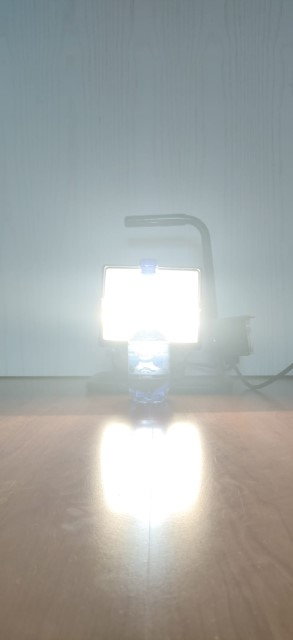
\includegraphics[width=0.30\textwidth]{Bilder/ueberbeleuchtet.jpeg}}\hfill
	\subfigure[normal]{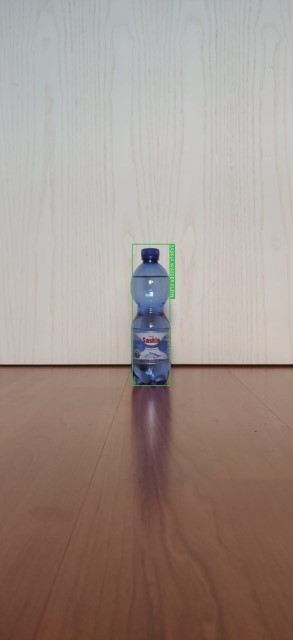
\includegraphics[width=0.30\textwidth]{Bilder/normalbeleuchtet.jpeg}}\hfill
	\subfigure[unterbeleuchtet]{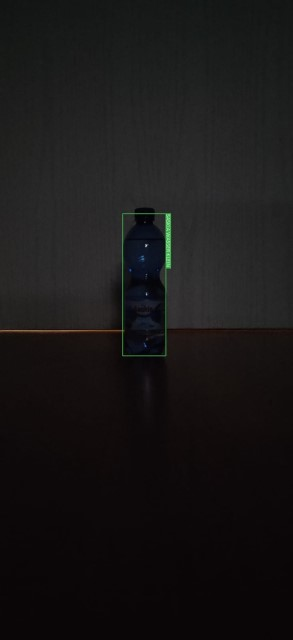
\includegraphics[width=0.30\textwidth]{Bilder/unterbeleuchtet.jpeg}}\hfill
	\caption{Detektionsverhalten bei unterschiedlichen Beleuchtungsverhältnissen}
	\label{sicht}
\end{figure}

Des Weiteren haben unterschiedliche Beleuchtungsgrade eine Auswirkung auf das Detektionsverhalten. In Abbildung \ref{sicht} wird unterschieden zwischen dem Detektionsverhalten bei überbeleuchteten, normalen und unterbeleuchteten Sichtverhältnissen. Überbeleuchtete Umgebungsverhältnisse erschweren die Objektdetektion in diesem Beispiel. 

Die Detektion reagierte allerdings invariant gegenüber unterschiedlichen Hintergründen oder Bildauflösungen.

\subsection*{YOLO}

Robin

\section{Drohnen Anbindung}

\subsection*{Drohnen Interface}

Robin, evtl. ein Grundlagenkapitel (war auch in Markus Feedback die Rede)

\subsection*{Modellinferenz}

Der Video Stream der Drohne kann mittels der \textit{openCV} Klasse \textit{VideoCapture} über das UDP Protokoll angesprochen werden. Bei der Inferenz fällt allerdings entgegen der Erwartungen auf, dass die Inferenz überdurchschnittlich langsam verläuft. Das Problem lässt sich auf die synchrone Arbeitsweise der bisherigen Detektionsalgorithmen zurück führen, bei dem erst ein neuer Frame des Videostreams angefragt wird, sobald das aktuelle Bild durch die Vorverarbeitung gelaufen ist und durch das Modell inferiert wurde. 

Um dem entgegen zu wirken, wurde ein Bufferkonzept in einem parallelem Thread realisiert, der einzelne Frames zeitgleich zur Inferenz anfragt und zwischenspeichert. Ist der Buffer voll, so werden nach dem \textit{First In First Out} Verfahren die älteren Frames verworfen. Dadurch konnte die FPS Anzahl von \textit{SSD} von maximal 18 auf die vollen 30 gesteigert werden. 

Ein weiteres Problem beschreibt die initiale Latenz zwischen der Inferenz und der Bildaufnahme. Die Inferenz kann erst gestartet werden, sobald die Gewichtungen des Modells initialisiert wurden. Dies lässt sich umgehen, indem entweder der Thread zur Bildaufnahme verzögern gestartet wird oder dessen Buffer kleiner gewählt wird.

+ Robin YOLO

\section{Dashboard Entwicklung}

Der Server wurde mit dem \textit{Flask} Framework in Python implementiert und läuft auf dem \textit{Web Server Gateway Interface} (WSGI) server \textit{Waitress}. Er führt den Inferenzalgorithmus des \textit{SSDs} bzw. des \textit{YOLO} Objektdetektors für jeden Frame des empfangenen Videostreams der Drohne aus und streamt die inferierten Bilder mit den Bounding Boxen an jeden Client. Der Client wurde mit dem \textit{Bootstrap} Framework designed (siehe Abbildung \ref{webapp}).

\begin{figure}[ht]
	\begin{center}
		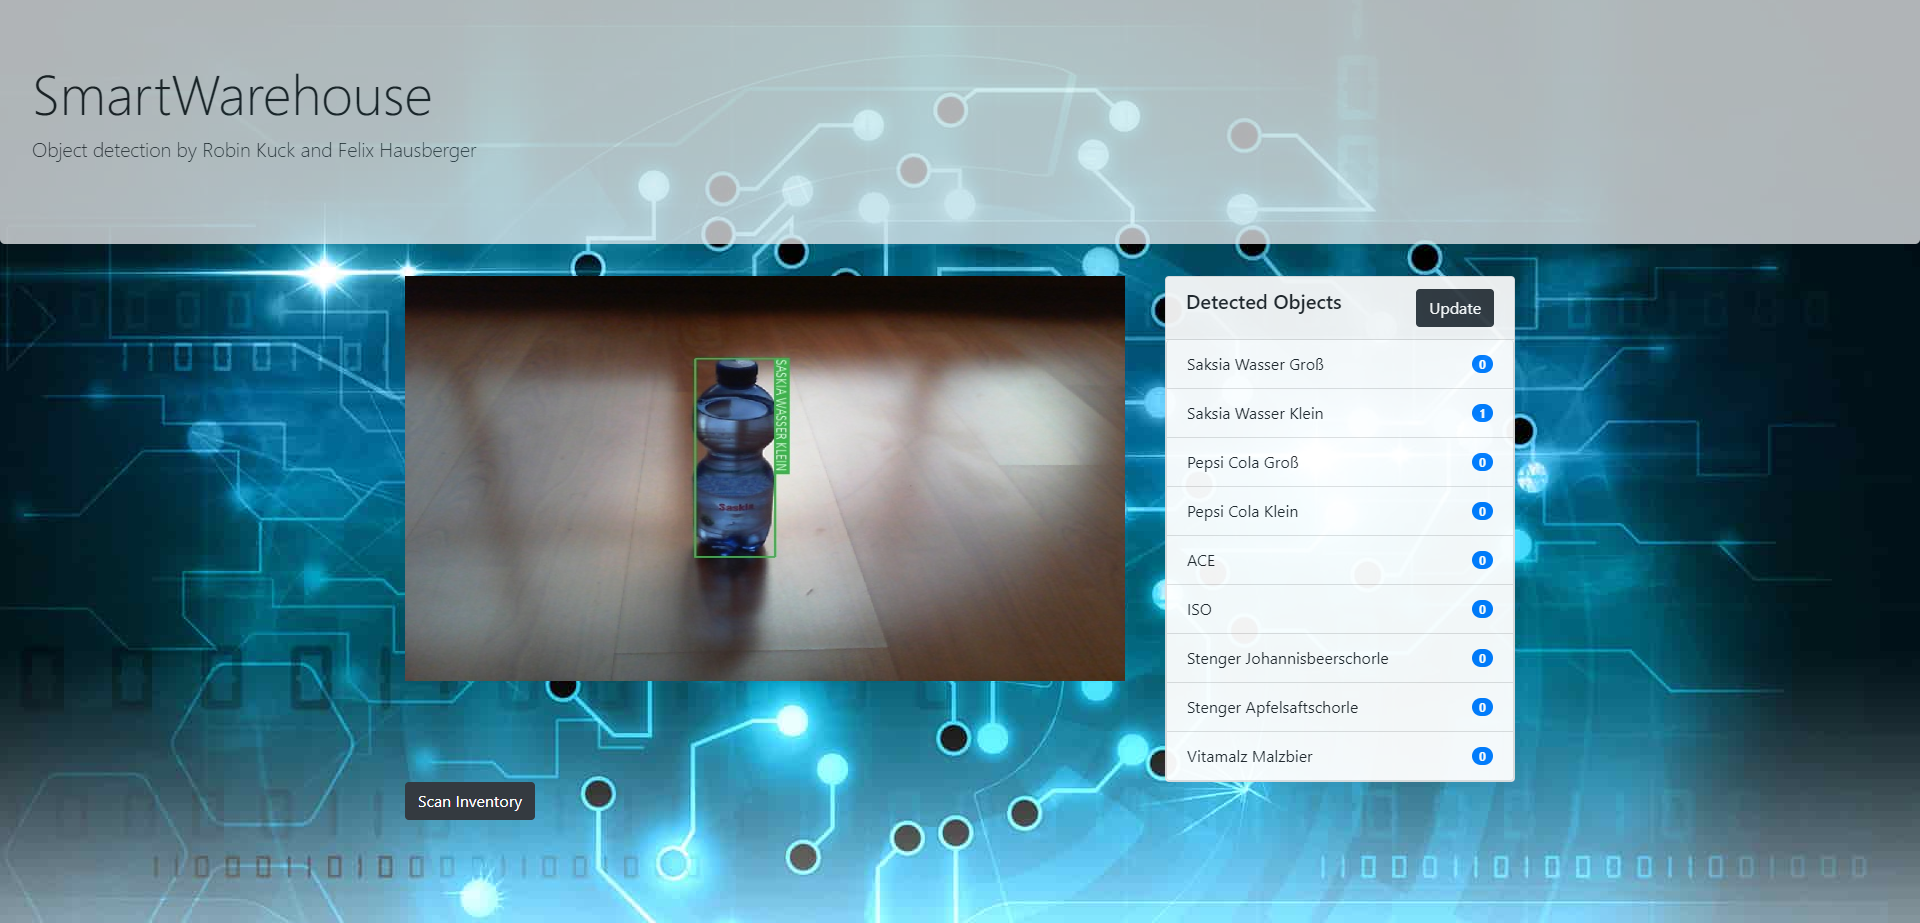
\includegraphics[width=15cm]{Bilder/webapp.jpeg} 
		\caption[Webapp SmartWarehouse]{Webapp SmartWarehouse}
		\label{webapp}
	\end{center}
\end{figure}

Auf Anfrage eines Client kann dieser die aktuell gezählten Objekte vom Server abfragen. Der Zählalgorithmus wird im folgenden Unterkapitel erklärt. 

\section{Zählalgorithmus}

\lstinputlisting[
label={code:formfield},
caption={Zählalgorithmus zum Zählen der detektierten Objekte},
captionpos=b,
basicstyle=\ttfamily\scriptsize,   
firstline=1,              
lastline=11                 
]{Quellcode/algorithmus.txt}

Der obige Algorithmus wird momentan dazu verwendet, um für das Industrieszenario einer Inventur einzelne detektierte Objekte zu zählen. Das Problem, dass der Algorithmus zu lösen versucht, enthält allerdings eine weitere Komplexitätsstufe. Dasselbe Objekt kann im Laufe der Inventur erneut auftreten und dessen relative Position im Bild ist ebenso variabel. In diesem Falle werden Objekte doppelt gezählt. 
